\newpage
\section{Projekt}

\subsection{Wybór technologii}

Dobór platformy sprzętowej rozpocząłem od zdecydowania się na korzystanie z techniki modulacji
LoRa. Poniżej przedstawiam krótki opis teoretyczny oraz uzasadnienie wyboru.

\subsubsection{Modulacja LoRa i technika Chirp Spread Spectrum}

LoRa (ang.\ \textit{Long Range}) to technika modulacji radiowej, która pozwala na przesyłanie
niewielkich pakietów danych na bardzo duże odległości - nawet kilkanaście kilometrów - przy
minimalnym zużyciu energii.\footnote{\url{https://www.gov.pl/web/instytut-lacznosci/lora-pod-lupa}}
Jej zamysł opiera się na technice modulacji CSS (ang.\ \textit{Chirp Spread Spectrum}) lub FSCM
(ang.\ \textit{Frequency Shift Chirp Modulation})~\cite{vangelista2017lora}. Polega ona na
kodowaniu sygnału przez cykliczne przesunięcie punktu startowego chirpa. Wspomniany chirp to
,,blok'' sygnału o liniowo zmiennej częstotliwości.

Modulację LoRa opisują trzy główne parametry:
\begin{itemize}
    \item \textbf{Współczynnik rozpraszania SF} (ang.\ \textit{Spreading Factor}) - określa
          liczbę chirpów przypadających na jeden symbol. Im wyższy SF, tym dłuższy czas transmisji
          symbolu, ale też lepsza czułość odbiornika i większy zasięg. W praktyce stosuje się
          wartości od 7 do 12.

    \item \textbf{Szerokość pasma BW} (ang.\ \textit{Bandwidth}) - określa zakres częstotliwości
          zajmowany przez sygnał. Szersza szerokość pasma oznacza krótszy czas transmisji symbolu
          przy tym samym SF, ale też wyższy poziom szumów i mniejszy zasięg. W praktyce do wyboru
          są częstotliwości 125, 250 lub 500~kHz.

    \item \textbf{Współczynnik kodowania CR} (ang.\ \textit{Coding Rate}) - określa nadmiarowość
          kodu korekcji błędów. Wyższy CR zwiększa odporność na błędy transmisji kosztem wydajności.
\end{itemize}

Przepustowość bitową modulacji LoRa wyraża wzór:\footnote{\url{https://josefmtd.com/2018/08/14/spreading-factor-bandwidth-coding-rate-and-bit-rate-in-lora-english/}}

\begin{equation}
    R_b = SF \cdot \frac{BW}{2^{SF}} \cdot \frac{CR}{4+CR}
    \label{eq:lora-bitrate}
\end{equation}

Kluczową zaletą CSS jest odporność na zakłócenia wąskopasmowe poprzez rozłożenie energii sygnału
na całe dostępne pasmo. Efekt Dopplera (istotny przy komunikacji w ruchu) również jest ograniczony.
Wynika to z tego, że odczyt symbolu polega w skrócie na mnożeniu odebranego sygnału przez chirp
bazowy i wykonaniu FFT (ang.\ \textit{Fast Fourier Transform}). Powstały w wyniku pik widmowy jest
jedynie przesunięty i przy prędkościach spotykanych w praktyce nie spowoduje błędu dekodowania.

Zazwyczaj do konfiguracji sieci Meshtastic używa się następujących parametrów: $SF=12$,
$BW=125$~kHz oraz $CR=4/8$. Podstawiając do wzoru~\ref{eq:lora-bitrate} osiągamy przepustowość
na poziomie 250~bps. Jest ona w zupełności wystarczająca do przesyłania krótkich pakietów
zawierających współrzędne GPS.

\subsubsection{Wybór platformy sprzętowej}

Rozważyłem możliwość wykorzystania różnych platform sprzętowych z modułami radiowymi LoRa:
\begin{enumerate}
    \item \textbf{Raspberry Pi z modułami LoRa} - mimo licznych zalet, takich jak bogate wsparcie,
          względnie wysoka moc obliczeniowa oraz elastyczność, przeważyły wady, które wykluczyły to
          rozwiązanie: zbyt duże zużycie energii, duże rozmiary, brak wodoszczelności. Podobne
          argumenty zdecydowały o wyeliminowaniu platformy \textit{Arduino~Uno/Nano z modułem LoRa}.
    \item \textbf{ESP32 z modułami LoRa} - w szczególności rozważałem \textit{Heltec ESP32 LoRa},
          czyli płytkę z wbudowanym modułem LoRa i wyświetlaczem OLED. Produkt ten posiada wiele
          cech wypełniających wymagania projektu (wbudowany moduł Bluetooth i LoRa, niskie zużycie
          energii, niski koszt), jednak nie są dostępne obudowy z zadowalającą wodoszczelnością
          i odpornością na uszkodzenia mechaniczne.
\end{enumerate}

Prowadząc badanie rynku modułów wykorzystujących LoRa do komunikacji, natknąłem się na platformę
Meshtastic. Jest to projekt OpenSource, który łączy firmware dla modułów radiowych LoRa
z ekosystemem aplikacji klienckich, tworząc zdecentralizowaną sieć mesh działającą w paśmie ISM
bez konieczności jakiejkolwiek infrastruktury zewnętrznej. Każdy węzeł sieci automatycznie
retransmituje pakiety innych węzłów, rozszerzając zasięg sieci wraz z liczbą urządzeń. Dodatkowo
projekt udostępnia publiczne API w postaci aplikacji Android
\texttt{com.geeksville.mesh}, eksportującej interfejs AIDL umożliwiający aplikacjom trzecim odczyt
danych telemetrycznych - w tym pozycji GPS węzłów.\footnote{\url{https://meshtastic.org/docs/development/firmware/build/}}
Sprzęt kompatybilny z Meshtastic jest ogólnodostępny i tani, a samo oprogramowanie bezpłatne.
Wybór padł na:
\begin{itemize}
    \item \textit{T-Beam} - popularna platforma oparta na ESP32 z wbudowanym modułem GPS, anteną
          LoRa oraz akumulatorem. Posiada duży akumulator oraz otwarte piny, które zostawiają
          szerokie pole manewru do rozwoju tego węzła w roli stacji bazowej.
    \item \textit{T-2000-E} - kompaktowe urządzenie oferujące wodoszczelność (IP67), wbudowany GPS
          oraz zoptymalizowaną żywotność baterii. Wymiary i kształt są najodpowiedniejsze do
          umieszczenia na obroży.
\end{itemize}

Otwartoźródłowy charakter projektu stwarza możliwość implementacji rozszerzeń dla węzłów sieci
w postaci modułów. Dzięki temu wybór Meshtastic jako platformy sprzętowej nie ograniczy projektu
do domyślnie dostępnych funkcji. Sporód dostępnych konfiguracji radiowych możemy wybrać parametry
dla modulacji LoRa. Są one zestawione w tabeli~\ref{tab:lora-presets}.\footnote{\url{https://meshtastic.org/docs/software/site-planner/}}

\begin{table}[!h]
    \caption{Predefiniowane ustawienia kanałów LoRa w Meshtastic}
    \label{tab:lora-presets}
    \centering
    \begin{tabular}{|l|c|c|c|}
        \hline
        \textbf{Ustawienie} & \textbf{BW [kHz]} & \textbf{SF} & \textbf{CR} \\
        \hline
        ShortTurbo   & 500 & 7  & 4/5 \\
        ShortFast    & 250 & 7  & 4/5 \\
        ShortSlow    & 250 & 8  & 4/5 \\
        MediumFast   & 250 & 9  & 4/5 \\
        MediumSlow   & 250 & 10 & 4/5 \\
        LongFast     & 125 & 11 & 4/5 \\
        LongModerate & 125 & 11 & 4/8 \\
        LongSlow     & 125 & 12 & 4/8 \\
        \hline
    \end{tabular}
\end{table}

Zwiększa to elastyczność projektu pod względem testów zajętości pasma w technice LoRa.

\subsubsection{Konfiguracja sieci Meshtastic}

Skonfigurowałem sieć Meshtastic, aby wszystkie węzły mogły przesyłać między sobą informacje
o swoim położeniu GPS.

\paragraph{Jak działa przesyłanie pozycji w Meshtastic.}

W sieci Meshtastic informacje o pozycji GPS są przesyłane jako część telemetrii węzła. Telemetria
jest automatycznie udostępniana wszystkim węzłom w sieci, które używają tego samego kanału PRIMARY
(lub kanału wtórnego z włączoną pozycją), mają zgodne ustawienia LoRa (częstotliwość, modem preset)
oraz są w zasięgu (bezpośrednio lub przez pośrednie węzły).

\paragraph{Konfiguracja - prywatne kanały.}

Ponieważ chciałem udostępniać pozycję tylko wybranym węzłom (tylko w mojej sieci), musiałem użyć
prywatnego kanału. Konfiguracja przebiegła następująco:

\begin{enumerate}
    \item \textbf{Wyłączyłem pozycję na kanale PRIMARY}:
          Settings $\rightarrow$ Radio Config $\rightarrow$ Channels $\rightarrow$ Channel 0 (PRIMARY)
          $\rightarrow$ Position Sharing: \textbf{WYŁĄCZONE}.

    \item \textbf{Utworzyłem prywatny kanał}:
          Settings $\rightarrow$ Radio Config $\rightarrow$ Channels $\rightarrow$ \textbf{Add Channel},
          z następującymi parametrami:
          \begin{itemize}
              \item \textbf{Channel Name}: \texttt{Reja}
              \item \textbf{PSK}: wspólny klucz szyfrowania
              \item \textbf{Position Sharing}: \textbf{WŁĄCZONE}
              \item \textbf{Position Precision}: najwyższy poziom precyzji 32-bity
                    (deklaruje dokładność co do metra)
          \end{itemize}

    \item \textbf{Dodałem ten sam kanał do wszystkich węzłów w grupie}: wszystkie węzły mają
          identyczną nazwę kanału \texttt{Reja} oraz identyczny klucz PSK.
\end{enumerate}

\subsection{Aplikacja mobilna MeshTracker}

\subsubsection{Architektura}

Aplikacja wykorzystuje architekturę opartą na wzorcu \textbf{MVVM
(Model-View-ViewModel)}\footnote{\url{https://learn.microsoft.com/pl-pl/dotnet/architecture/maui/mvvm}}
z osobnymi, dodatkowymi warstwami odpowiedzialnymi za komunikację zewnętrzną z aplikacją Meshtastic.
Jest to standardowo wykorzystywany wzorzec, który oddziela logikę działania aplikacji od interfejsu
użytkownika.

\begin{figure}[!h]
    \caption{Architektura aplikacji MeshTracker}
    \label{fig:architektura}
    \centering
    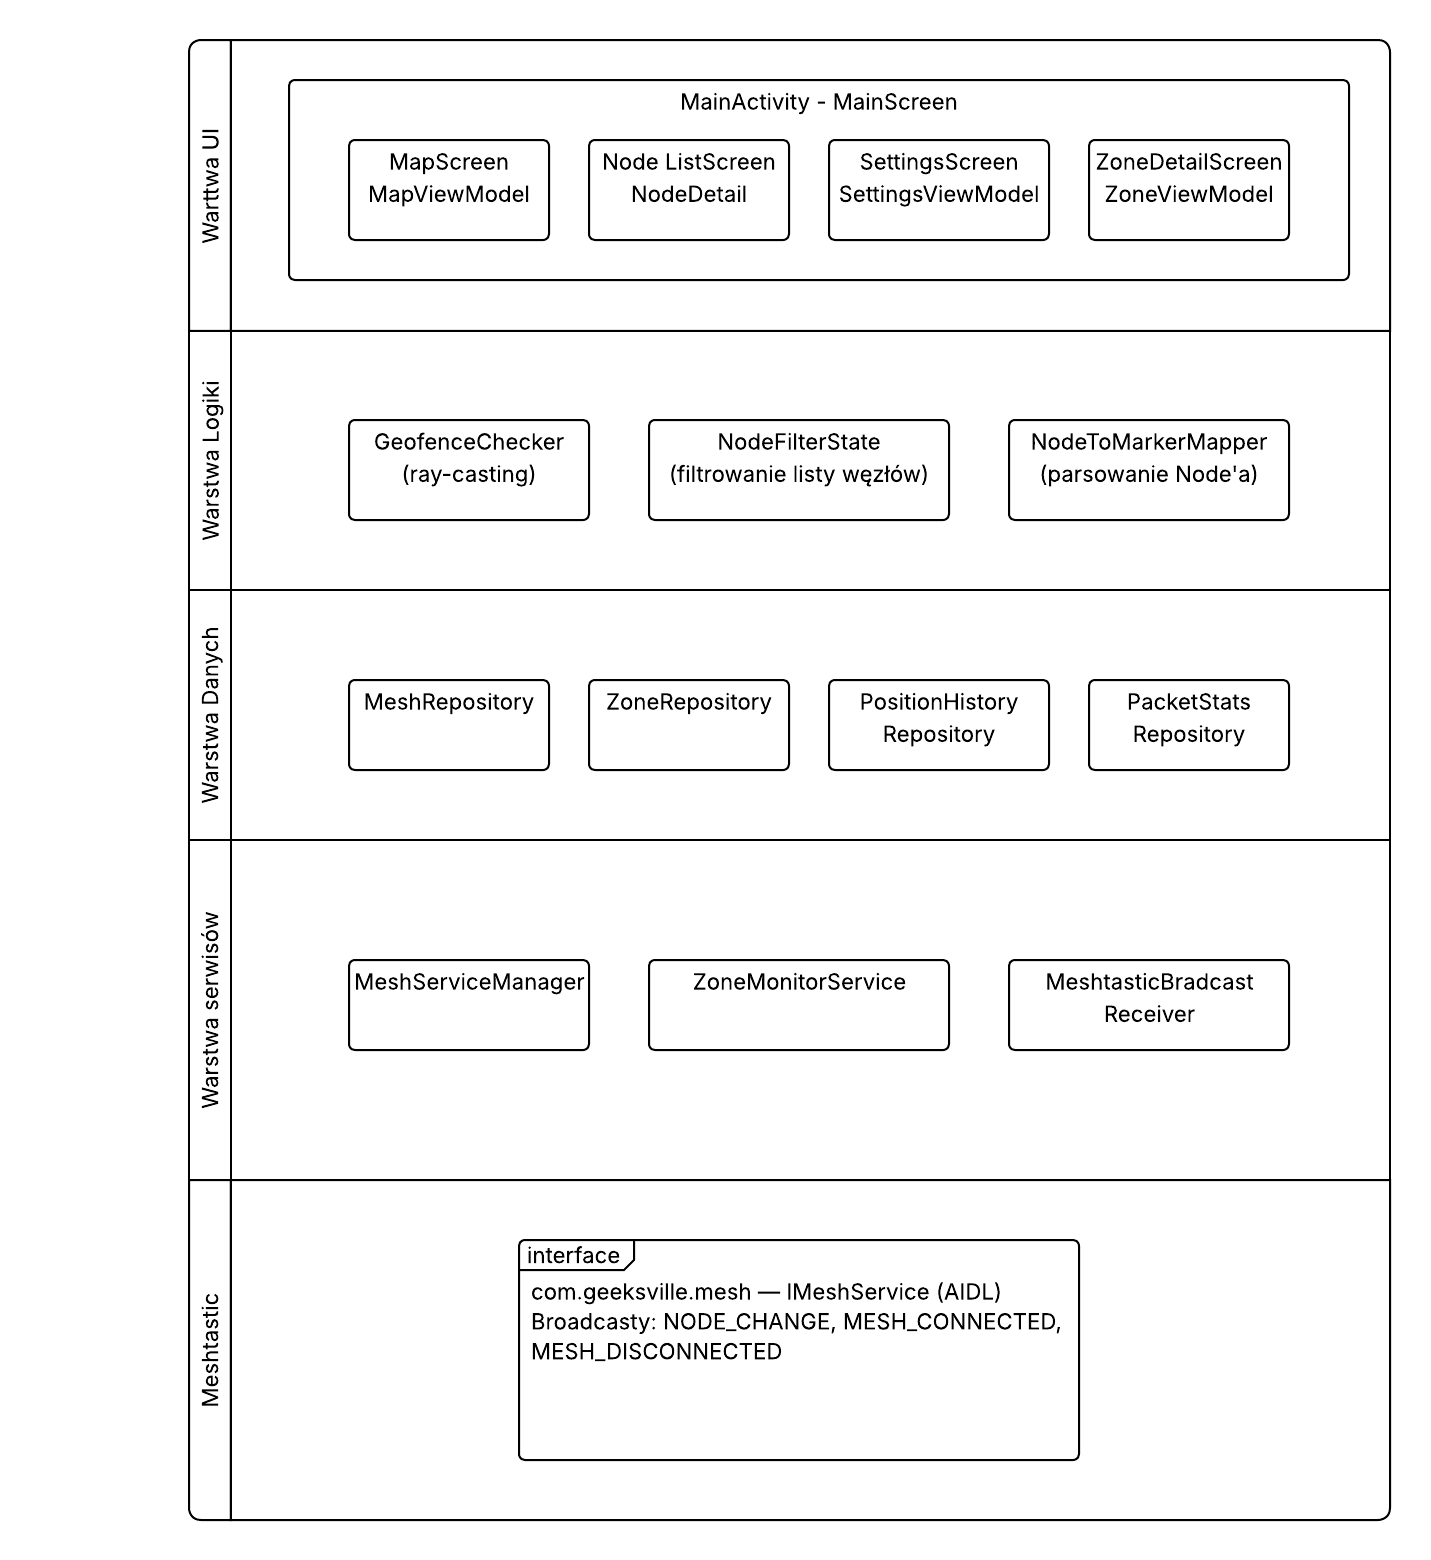
\includegraphics[width=0.9\linewidth]{ArchitectureWhiteBackground.png}
\end{figure}
